\chapter [Performance Comparison of Modulation Scheme-BASK]{Performance Evaluation of Modulation Scheme-BASK}


\section{AIM}

Implement a digital modulation scheme (BASK) using Scilab. Add noise of different SNR level to model a transmission channel. Demodulate it and find BER for each case and plot it. Compare it with theoretical model.


\section{THEORY}

Digital data with binary values are modulated and represented as the binary amplitude of a sinusoidal carrier in BASK signalling scheme. The decoding will be erroneous if additive noise disrupts the modulated signal during transmission. The bit error rate (BER) decreases with increase in Signal to Noise Ratio (SNR). 

The following experiment compares the theoretical relation between the two with simulated values of BER. Noise corresponding to different values of SNR is added to the modulated signal and the resulting signal is used for message detection. The demodulated message is then compared with the actual message to find the BER corresponding to each value of SNR(2 dB, 4 dB, 6 dB, 8 dB, 10 dB).

\section{PROCEDURE}

\paragraph{}
\begin{enumerate}
\item
Start Scilab on PC and Scilab console window opens. Create a new blank SciNote.
\item
The code for the required program is typed and saved as Scilab SCE file with an extension .sci
\item

The continuous plots are made using the function $plot$ and discrete plots are made using the function $plot2d3$ with the corresponding x axis and y axis variables written inside paranthesis.

\item
To view all the plots in the same window the function $subplot$ is used.
\item
The results and the errors in the program are displayed in the console window.
\item
Figures in every figure window is plotted using $xs2pdf$ function.
The typed program is run using the “execute”.
\end{enumerate}

\section{SCILAB CODE}

\subsection*{Comparison of BER performance for different SNR levels for BASK}
\lstinputlisting[caption=Comparison of BER performance for different SNR levels for BASK]{./scilabCode/berbask.sci}



\section{RESULT}
Performance evaluation plots were implemented.

\begin{figure}
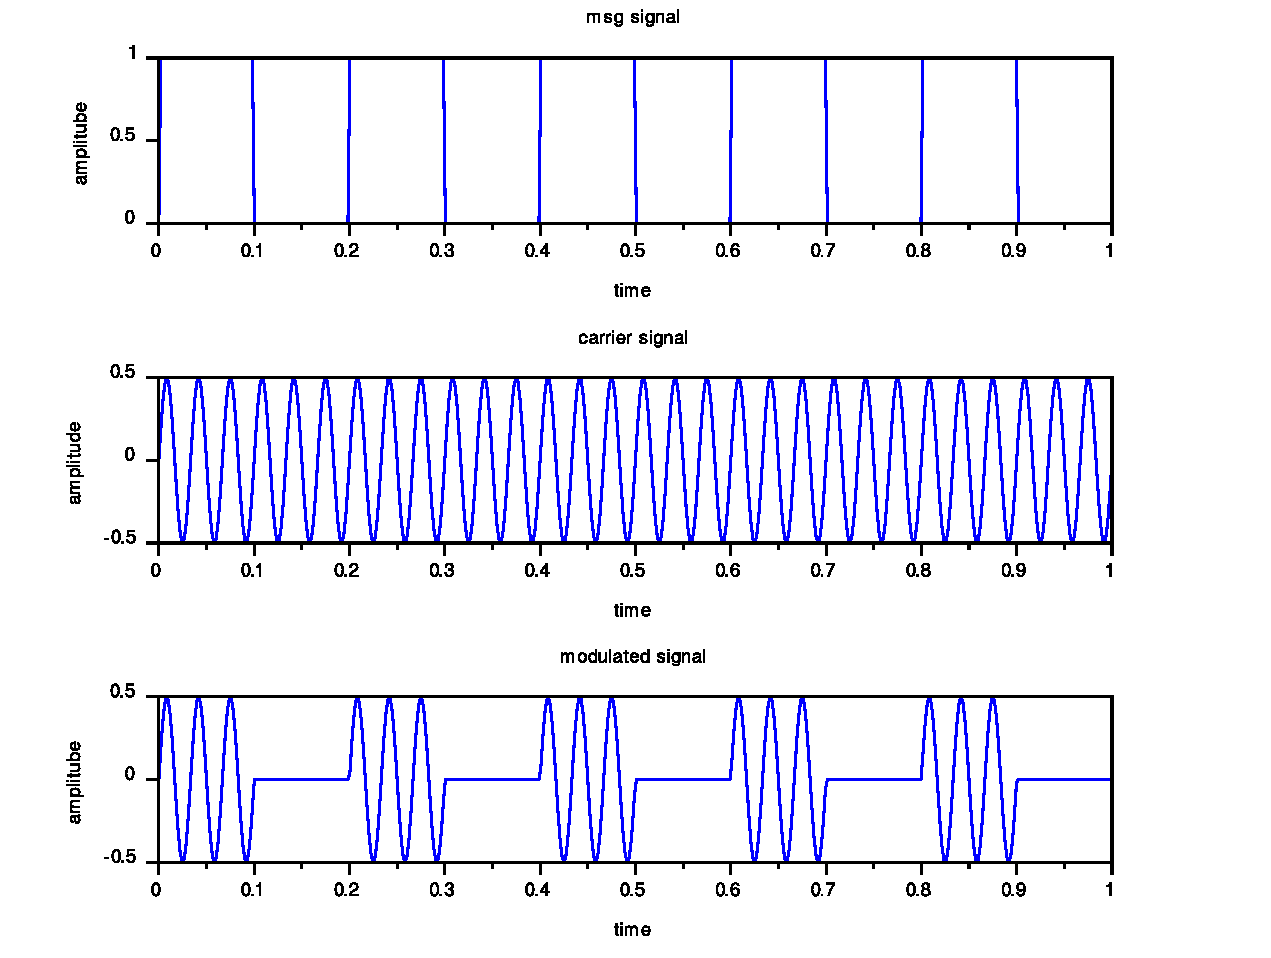
\includegraphics[scale=.7]{/home/kavya/kavyadev/DSPlab/scilabCode/TransmissionASK.pdf}
\caption{Plot of message signal, carrier and BASK}
\label{transmissionask}
\end{figure}


\begin{figure}
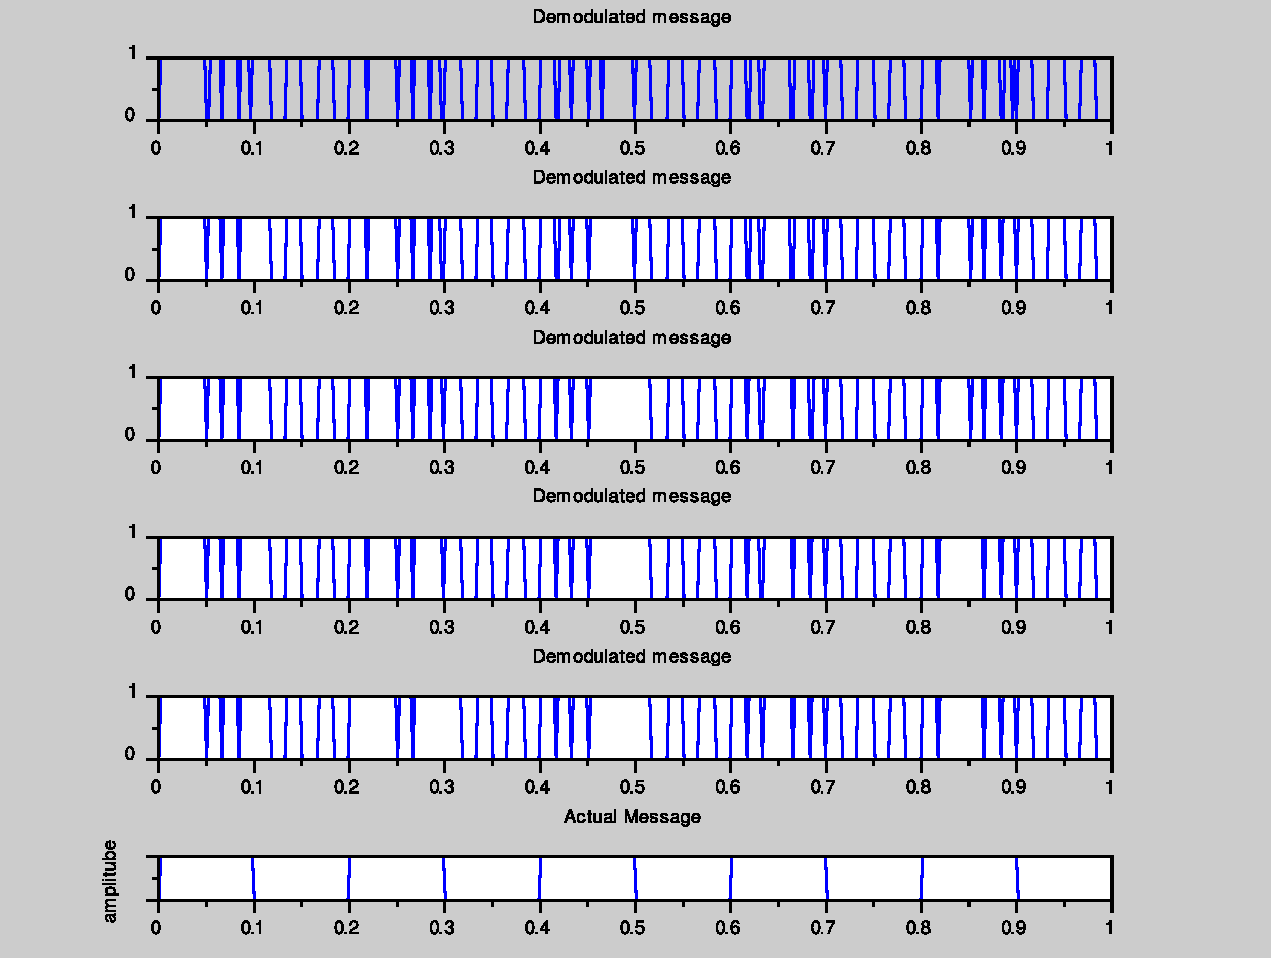
\includegraphics[width=\textwidth, height=15cm]{/home/kavya/kavyadev/DSPlab/scilabCode/ReceptionASK.pdf}
\caption{Plot of demodulated signals corresponding to different SNR}
\label{receptionask}
\end{figure}


\begin{figure}
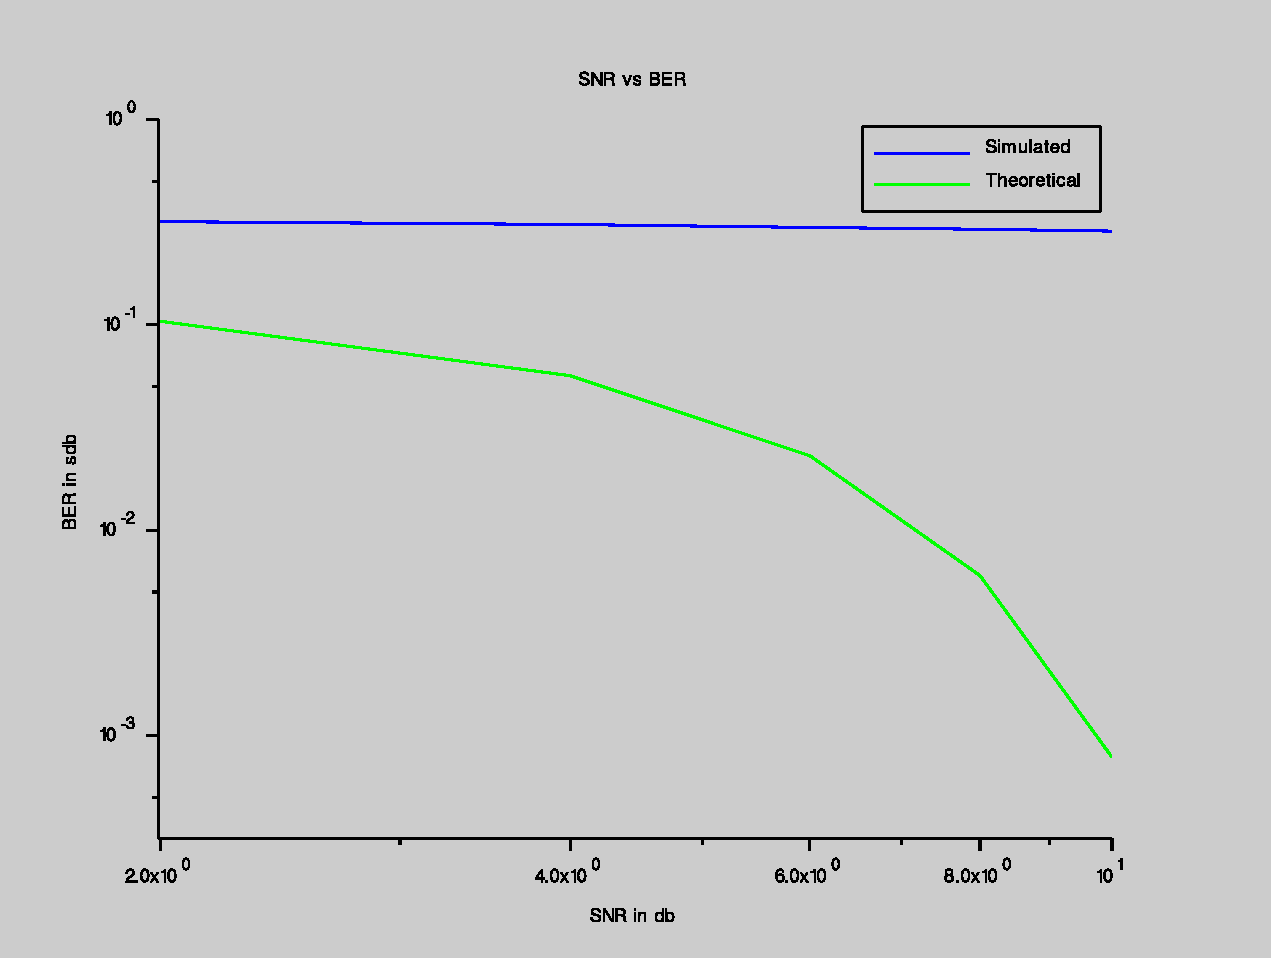
\includegraphics[scale=.7]{/home/kavya/kavyadev/DSPlab/scilabCode/BERVsSNRASK.pdf}
\caption{Plot of BER Vs SNR (Theoretical and Simulated)}
\label{BER Vs SNR}
\end{figure}
